\section{Systematic Uncertainties}

The systematic uncertainties of the oscillation measurement consists of uncertainties on the properties of the detector, the neutrino flux, neutrino cross-sections, and atmospheric muon background. The effects of each of these uncertainties on the expectation values of the analysis histogram are parametrized by several parameters that are included as nuisance parameters during the fit with gaussian priors where external constraints are available. 

\subsection{Detector Properties}
\label{sec:detector-unc}
Systematic uncertainties on the detector properties that need to be taken into account are the overall optical efficiency of the DOMs as well as the properties of the surrounding ice. The parametrization and priors of each of these properties are informed by IceCube calibration studies. 
\begin{itemize}
    \item DOM efficiency: A factor that scales the probability that a photon hitting the PMT of a DOM will produce a photo-electron that is measured by the electronics. Nominal value is 1, prior standard deviation is 10\%.
    \item Hole ice: The ice within the column where the holes for the strings have been drilled has different optical properties from the surrounding ice. The effect of this difference is modelled as a variation of the angular acceptance of the DOMs. A Principal Component Analysis was run on several pre-existing models of the angular acceptance curves to find a generic parametrization of their differences. In this analysis, we scale the two most important Principal Components to model the effect of hole ice on the histogram. There are no priors on those components and they are allowed to vary within the range covered by the produced systematic sets plus a small amount of extrapolation.
    \item Bulk ice: The over-all absorption and scattering coefficients of all ice layers are multiplied by a scaling factor. The nominal value for ice absorption is 1.0 with a prior standard deviation of 5\%. The nominal value for ice scattering is 1.05 with a prior standard deviation of 10\%.
\end{itemize}

In total, the uncertainties on the detector properties is modeled by five  parameters, one for the DOM efficiency, two for the hole ice model and two for the bulk ice uncertainty. To model the effect of these parameters on the analysis histogram, several MC sets at different variations of DOM efficiency, hole ice, and bulk ice parameters are produced. These MC sets are used to find a parametrization that will model how the distribution of events in energy, zenith and PID will change as a function of these parameters as described in the following section.

\subsubsection{Method of bin-wise linear fits}
\label{sec:hypersurfaces}
\begin{marginfigure}[\baselineskip]
    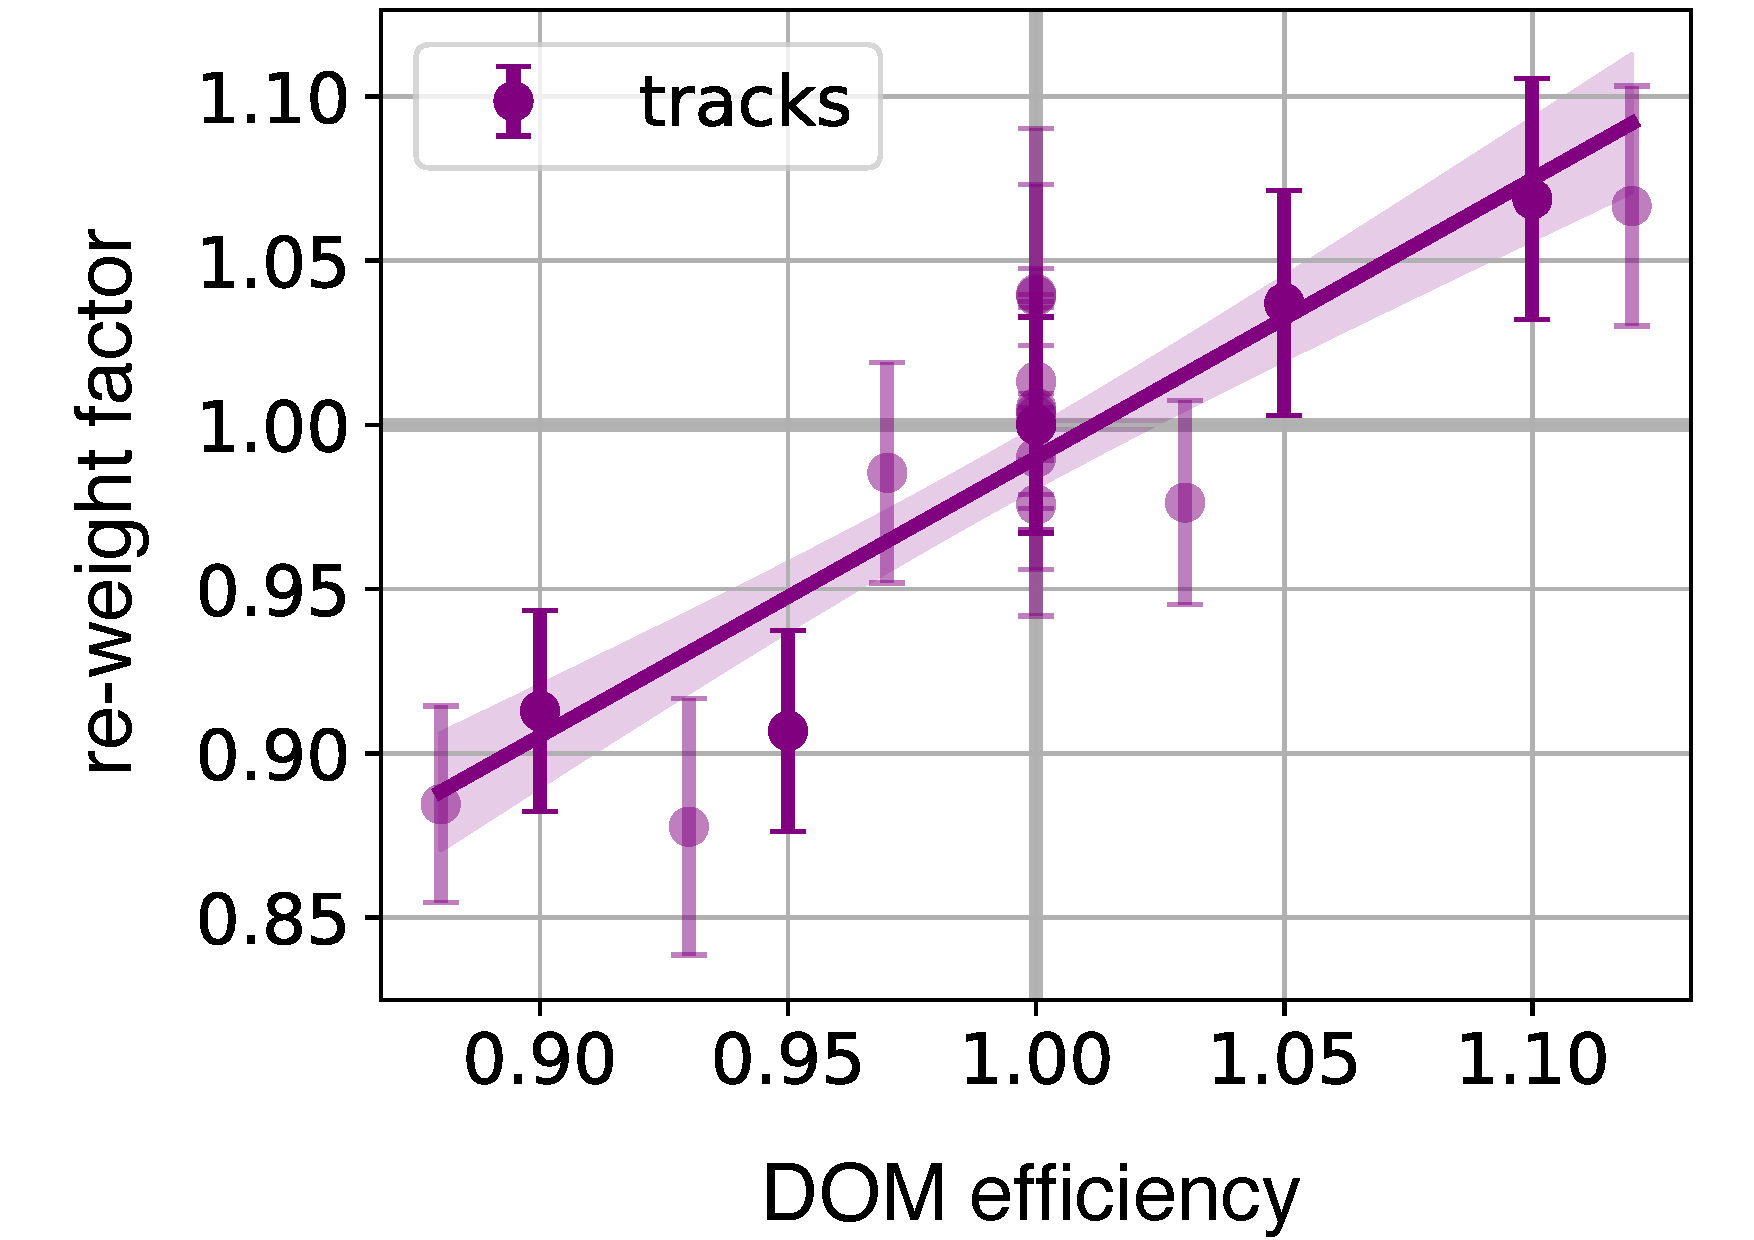
\includegraphics[width=\linewidth]{figures/measurement/systematics/detector/hypersurface_example_v2.pdf} 
    \caption{Example of a linear regression in one bin of the analysis projected onto the dimension of the DOM efficiency. Data points with translucent error bars originate from MC sets where one or more parameters besides DOM efficiency are at off-nominal points and are projected along the fitted surface to the nominal point.}
    \labfig{hypersurface-example-fit}
\end{marginfigure}
For the standard three-flavor fit, the method adopted to model systematic detector uncertainties is an extension to the same method that has been used in previous IceCube oscillation studies\cite{IceCube:2019dqi}. The expectation value of the analysis histogram is calculated using each of the discrete MC sets with varied detector properties, and the expectation values in every bin are divided by the expectation given by the nominal MC set. Then, a linear least-squares regression is performed for every bin in the histogram to model the expectation value as a function of all five parameters, resulting in five gradients and one intercept value for every bin. The result of one such fit for an arbitrarily chosen bin is shown in \reffig{hypersurface-example-fit}. A side effect of this process is that the intercept of the linear regression has a much smaller statistical uncertainty than the statistical uncertainty of the nominal MC set alone, which reduces the statistical MC uncertainty of the analysis over-all.

\begin{figure}
    \centering
    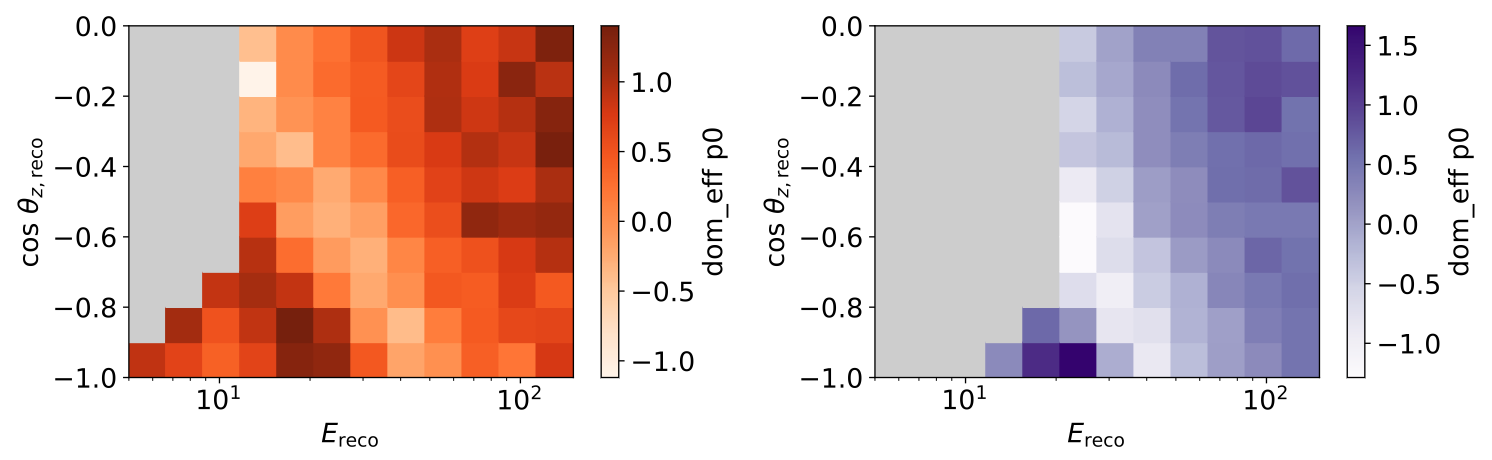
\includegraphics[width=0.9\linewidth]{figures/measurement/systematics/detector/dom_eff_slopes.png}
    \caption{Gradient of the relative bin count with respect to DOM efficiency.}
    \label{fig:dom-efficiency-slopes}
\end{figure}
A fundamental weakness of linear fit treatment is that the fitted parameters are only valid for the  choice of oscillation and flux parameters that they have been fit with. In particular, there is a strong interaction between the DOM efficiency parameter and the $\Delta m^2_{31}$ oscillation parameter. As can be seen in \reffig{dom-efficiency-slopes}, the gradients of the relative bin counts with respect to DOM efficiency show a distinct imprint of the oscillation minimum. However, the location of this minimum depends on the current value of $\Delta m^2_{31}$, which causes a considerable bias if the value of $\Delta m^2_{31}$ at which the gradients are to be evaluated is different from the value at which they have been fit. This is mitigated by running the fits at several values of $\Delta m^2_{31}$ covering the entire plausible range of this parameter, and interpolating all fit parameters with a piece-wise linear function between those points. As a result, all slopes and intercept values change as a function of the mass splitting. While the interactions between detector systematic uncertainties and analysis parameters are not limited to the mass splitting, the bias produced due to the choice of other parameters was found to be much smaller and is therefore neglected in the three-flavor analysis. 

\subsubsection{Method of likelihood-free inference}
\label{sec:ultrasurfaces}
 As described in \refsec{hypersurfaces}, the gradients acquired by bin-wise linear regressions in the analysis histogram are only correct for the particular choice of flux and oscillation parameters at which they have been fit. For the three-flavor analysis, this can be mitigated by a piece-wise interpolation of the gradients as a function of the mass splitting $\Delta m^2_{31}$, and the impact of other parameters is small enough that this one-dimensional interpolation is sufficient. However, for the sterile analysis, several additional oscillation parameters have the potential to substantially change the shape of the oscillation pattern and therefore change the detector response in each bin. The grid required to apply the interpolation to all potentially relevant parameters would have to have at least five dimensions and the RAM requirement to hold all those parameters would have been prohibitive. It was therefore deemed necessary to develop an entirely new method for the treatmetn of detector systematic uncertainties that entirely decouples the detector response from flux and oscillation weights that is described in this section.

The goal of this treatment of detector systematic effects is to find re-weighting factors for every event in the nominal MC set that correspond to how much more or less likely that particular event would be if the detector properties were different. These re-weighting factors should be independent from any other event weights, especially flux and oscillation weights. To get an intuition, one may look at an event in which the reconstructed energy is larger than the true energy. Such an event is more likely to occur when the DOM efficiency is higher than nominal, and less likely when the DOM efficiency is lower than nominal. This relationship will not change depending on the initial flux of the primary neutrino or oscillation effects, because the detector only reacts to the final state.

Using the discrete MC sets with different variations of detector parameters, one needs to find the re-weighting factors, $R_{ik}$, for each event in the nominal MC set, $i$, such that re-weighting every event by its weighting factor produces the same distribution in energy, zenith angle and PID as the off-nominal MC set, $k$. If the true distributions of event parameters in each MC set was known, this weighting factor could be calculated as the ratio
\begin{equation}
    R_{ik} = \frac{P(X_i|\theta_k)}{P(X_i|\theta_{\rm nominal})} \frac{P(\theta_k)}{P(\theta_{\rm nominal})}\;, \label{eq:ratio-likelihood}
\end{equation}
where $X_i$ are the parameters of the event, and $\theta_k$ are the detector parameters of the off-nominal MC set, $k$. The probability distribution $P(X_i|\theta_k)$ is the distribution of the event parameters in MC set $k$, and $\theta_{\rm nominal}$ contains the values of the detector parameters of the nominal MC set. The second fraction is the ratio of the total normalization of events under different detector parameter values. For instance, if an increase in DOM efficiency increases the total number of events by 10\%, then $P(\theta) / P(\theta_{\rm nominal}) = 1.1$.

In practice, of course, the probability distributions $P(X_i|\theta_k)$ is unknown, but the factors $R_{ik}$  can still be extracted from the available MC sets.
The first step is to apply Bayes' theorem to express $R_i$ as the ratio of the posterior probability distribution of the detector parameters given the event parameters,
\begin{equation}
    R_{ik} = \frac{P(\theta_k|X_i)}{P(\theta_{\rm nominal}|X_i)}\;. \label{eq:ratio-posterior}
\end{equation}
The posterior distributions, $P(\theta_k|X_i)$, can be acquired from a classifier trained to give the posterior probability for an event with parameters $X_i$ to belong to MC set $k$. This means that the task of finding the re-weighting factors can be translated into a \emph{classification task}. Such an inference method, where probability distributions are learned as a ratio of posteriors from a classifier, is also known as a \emph{likelihood-free inference} method.

\subsubsection{K-Neighbors method to calculate posteriors}
In principle, any classifier that provides well-calibrated posterior outputs can be plugged into eq.~\ref{eq:ratio-posterior}. For this analysis, the simple and robust \emph{k-neighbors} method is used.
The K-Neighbors classifier calculates posterior probabilities by finding the set $\mathcal{N}$ of the $N$ nearest neighbors for every event, $i$. This set is defined as the set of $N$ events with the smallest Euclidean distance in the event parameters $X$.  Then, the estimate for the posterior for set $k$ is the fraction of the total weight of the neighbors belonging to set $k$,
\begin{equation}
    P(\theta_k|X_i) = \frac{\sum_{j\in{\mathcal{N}\cup k}} w_j }{\sum_{j\in{\mathcal{N}}} w_j}\;. \label{eq:posterior-knn}
\end{equation}
The weights $w_j$ are the weighted effective area that every simulated MC event corresponds to and correct for the different amount of MC that was produced for every systematic MC set. They do not include neutrino flux or oscillation effects.

While this method is very robust, it is also prone to over-fitting if the number of neighbors is chosen to be too small. On the other hand, if the number of neighbors is too large, it might blur out important features and under-fit. An increased number of neighbors also causes a systematic bias in the probability estimate due to the fact that the distribution across the selected neighbors is not perfectly uniform. This bias is corrected to linear order by re-weighting the events in each neighborhood as described in appendix \ref{apx:knn-correction}. With this bias correction applied, a neighborhood size of 200 per included MC set was found to be a good compromise between bias and overfitting.

\subsubsection{Classification variables}
The input variables passed into the classifier for each event, $X_i$, need to cover all variables that are used in the binning ($E_{\rm reco},\cos(\theta_{\rm reco}),{\rm PID}$) as well as all variables that are used when re-weighting events by flux and oscillation probabilities ($E_{\rm true},\cos(\theta_{\rm true})$)\footnote{Even if other variables can in principle influence the detector response, they do not have to be included as long as their distribution does not change. See also appendix \ref{apx:implicit-marginalization}.}. This gives a total of five input variables that are used for classification. Because the K-neighbors classifier calculates euclidean distances between events in these five dimensions to determine which events are neighbors, all dimensions are transformed to be approximately normally distributed as follows and then scaled to have a unit variance:
\begin{itemize}
    \item Energies are replaced by their logarithm
    \item The zenith angle is used directly, rather than its cosine
    \item The PID, which is the probability output of a BDT, is transformed into the log-odds ratio, $\mathrm{LOR}=\log({\rm PID}) - \log(1-{\rm PID})$. This transformed variable turns the pileup of events near a PID value of one into a long tail.
\end{itemize}
The classifier is fit on the transformed variables separately for each flavor for CC interactions, and the combined set of all NC interactions.

\subsubsection{Calculating event-wise gradients}

The K-Neightbors calculation produces event weights that can re-weight the events of the nominal MC set to imitate the distribution of any other MC set. To be useful in an analysis, however, it is a requirement that this re-weighting can be interpolated to any value of detector parameters between the discrete MC sets. This is accomplished by fitting a vector of gradients, $g_i$, for every event, by minimizing the negative log-likelihood
\begin{equation}
    -\log\mathcal{L} = -\sum_k P_{\rm obs}(\theta_k | X_i) \log P_{k, \rm pred}(g_i, X_i)\;, \label{eq:grad-nllh}
\end{equation}
where the observed probability is $P_{\rm obs}(\theta_k | X_i)$ from the K-neighbors calculation and the  predicted probability $P_{k, \rm pred}(g_i, X_i)$ is
\begin{equation}
    P_{k, \rm pred}(g_i, X_i) = \frac{\exp(\sum_j \theta_{k,j} g_{i,j})}{\sum_l\exp(\sum_j \theta_{l,j} g_j)}\;.
\end{equation}
The motivation for the negative log-likelihood loss in eq.~\ref{eq:grad-nllh} is that minimizing this quantity is equivalent to minimizing the cross-entropy between labels $P_{\rm obs}$ and class predictions  $P_{k, \rm pred}$, and it has been shown that classifiers that minimize the cross-entropy end up learning posterior distributions\cite{NNPosteriors}.

To model non-linear effects, gradients are fit not only to the five detector parameters, but also to their squared values, for a total of ten gradients per event.

\subsubsection{Evaluation}
Once the event-wise gradients for all detector uncertainty parameters have been obtained, all events can be easily re-weighted during a fit for any given set of detector parameters, $\theta$, by multiplying the weight for each event by the ratio
\begin{equation}
    R_i(\theta)=\frac{P(\theta|X_i)}{P(\theta_{\rm nominal}|X_i)}=\exp\left(\sum_j (\theta_j - \theta_{j, \rm nominal}) g_{ij}\right)\;.\label{eq:ultrasurf-eval}
\end{equation}

\subsubsection{Performance}
To verify that the re-weighting according to eq.~\ref{eq:ultrasurf-eval} gives the expected result, they are used to reproduce each systematic MC set and calculate the bin-wise pulls between the reproduction and the systematic set. When the gradients are correct, the pull between the set and its reproduction,
$$p_n = \frac{N_{\mathrm{reprod}, i} - N_{\mathrm{syst}, i}}{\sqrt{\sigma^2_{\rm nominal} + \sigma^2_{\rm syst}}}\;,$$
should follow a standard-normal distribution. Fig.~\ref{fig:ultrasurf-binwise-pulls} shows the result of this test for the four MC sets in which only the DOM efficiency is varied between 90\% and 110\% percent. The spread of the bin-wise pulls closely follows a normal distribution standard deviation of one, as expected, but the total normalization is slightly under-estimated for the MC set 0004 with DOM efficency of 110\%. This is not too concerning for this analysis, since the total normalization is a free parameter without a prior. A similar performance is found for all included MC sets. 

Fig.~\ref{fig:dom-eff-prediction} shows the prediction of the bin count as a function of the DOM efficiency scale, $\epsilon_{\rm DOM}$ at the nominal point (left panel) and for different injected values of the mass splitting $\Delta m^2_{31}$ (right panel) for one arbitrarily chosen bin of the analysis. The prediction matches the shape of the bin count change very well, although it is offset slightly towards lower bin counts. This is expected, since the prediction is based on re-weighting the nominal MC set events without any corrections on the bin count at the nominal point. The error band shown in the figure corresponds to the uncertainty of the nominal set. The right panel of Fig.~\ref{fig:dom-eff-prediction}, demonstrates that the prediction automatically adjusts itself to any injected value of oscillation parameters. This happens despite the fact that the flux and oscillation weights have not been used at all when fitting the event-wise gradients, which demonstrates that the detector response has truly been decoupled from flux and oscillation effects. 

\begin{figure}
    \centering
    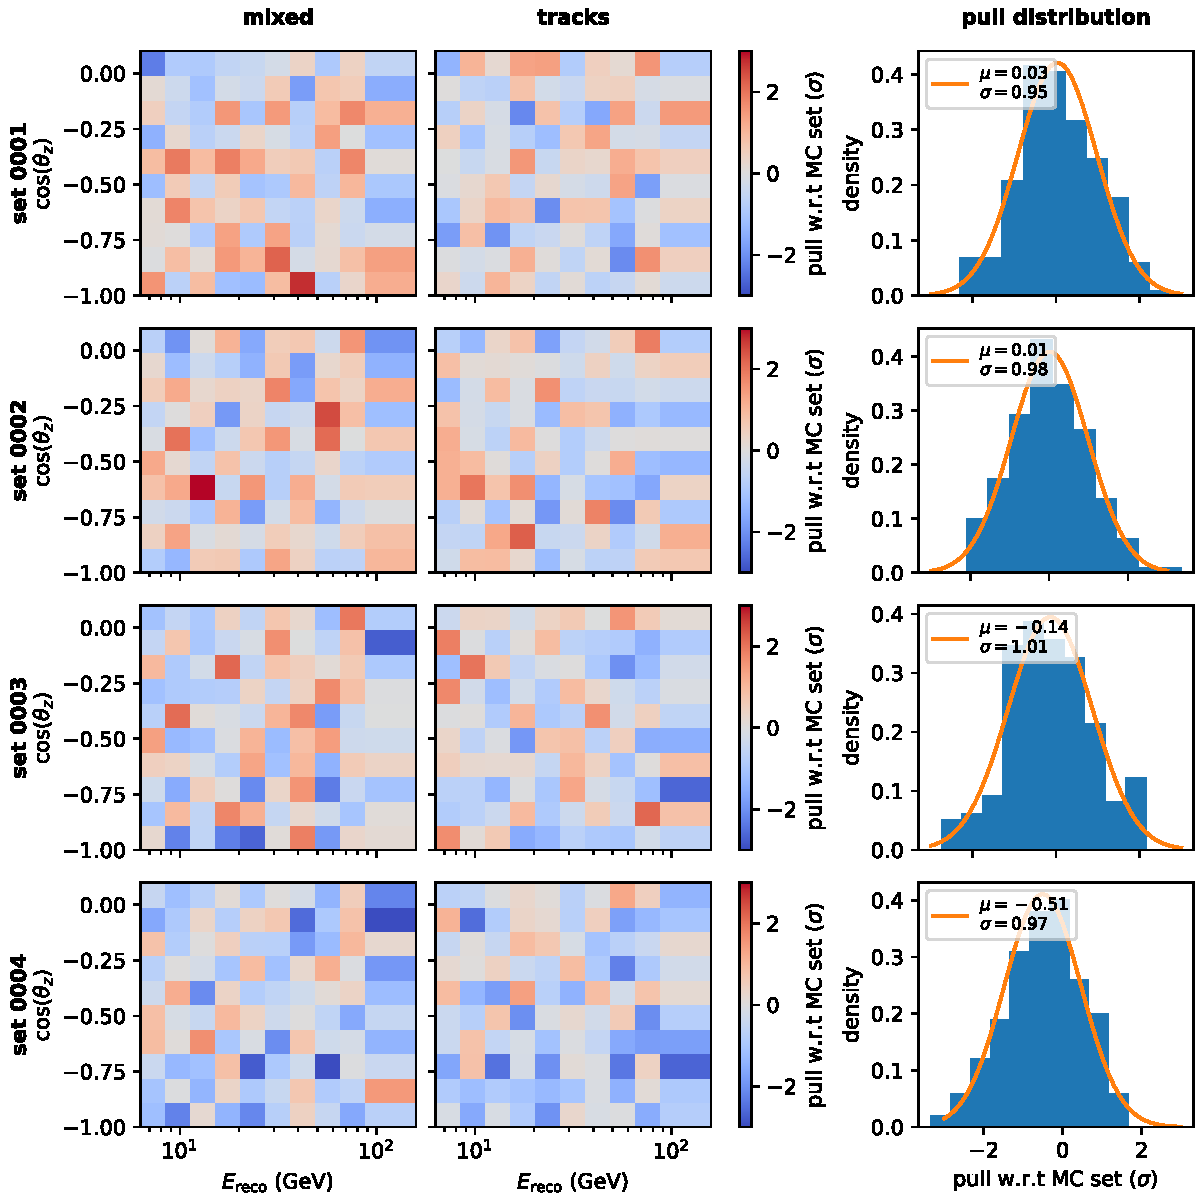
\includegraphics[width=0.9\textwidth]{figures/measurement/systematics/detector/ultrasurface_performance_vs_blind_fits_domeff_sets.pdf}
    \caption{Binwise pulls between the nominal set after re-weighting according to eq.~\ref{eq:ultrasurf-eval} and the systematic MC sets 0001, 0002, 0003, and 0004 representing DOM efficiency values of 90\%, 95\%, 105\%, and 110\%, resepctively. The 1D histogram in each row shows the distribution of the pulls over all bins.}
    \label{fig:ultrasurf-binwise-pulls}
\end{figure}

\begin{figure}
    \centering
    \begin{subfigure}{0.45\textwidth}
        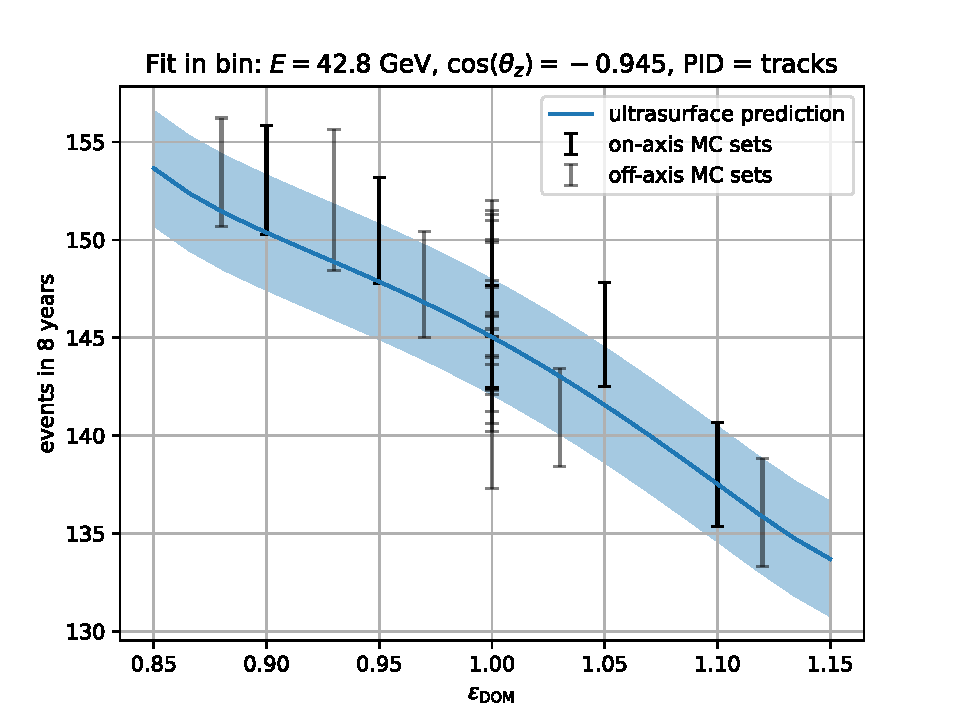
\includegraphics[width=\textwidth]{figures/measurement/systematics/detector/dom_eff_prediction.pdf}
        \caption{Prediction at best fit point of three-flavor analysis}
    \end{subfigure}
    \hfill
    \begin{subfigure}{0.45\textwidth}
        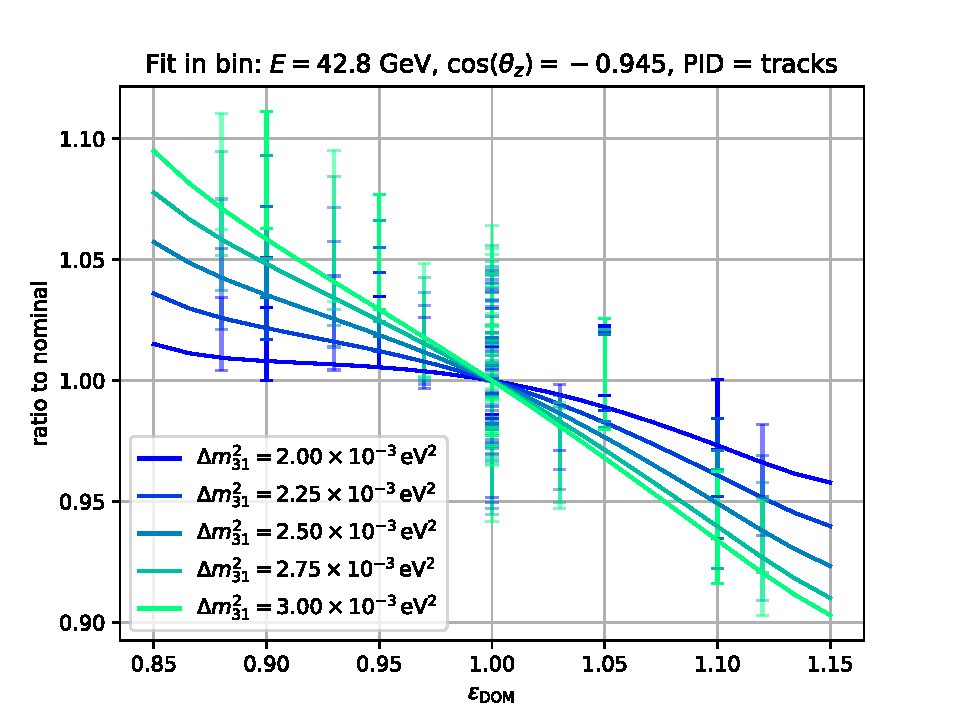
\includegraphics[width=\textwidth]{figures/measurement/systematics/detector/dom_eff_mass_splitting_scan.pdf}
        \caption{Prediction at different mass splitting values.}
    \end{subfigure}
    \caption{Prediction of bin counts in one bin of the analysis as a function of the DOM efficiency scale, $\epsilon_{\rm DOM}$. The error band in the left panel corresponds to the error on the nominal MC prediction without errors on the event-wise gradients.}
    \label{fig:dom-eff-prediction}
\end{figure}

\subsection{Atmospheric Neutrino Flux}
\label{section:flux_systs}

The atmospheric neutrino flux can vary depending on the choice of primary cosmic ray (CR) model, assumed meson yield, hadronic interaction (HI) model and atmospheric density model that are used in the calculation. This analysis uses the HKKM model as the baseline flux model and calculate the variation to the overall flux using \href{https://github.com/afedynitch/MCEq}{MCEq version 1.1.3}. The nominal flux, $\Phi_{\rm nom}$, is modified to a systematic flux, $\Phi_{\rm sys}$, so that

$$\Phi_{\mathrm{sys}} = (\Phi_{\mathrm{nom}} \cdot \Delta \Phi_{\mathrm{nom}}) + \bigg( b \cdot \frac{\mathrm{d} \Phi_{\mathrm{nom}}}{\mathrm{d}B} \bigg)$$

The first term is due to the CR flux uncertainty and corresponds to shifting the spectral index of the neutrino flux, with a pivot point at 24 GeV. The uncertainty on meson production is included in the last term, where $b$ is the magnitude of the uncertainty and $ {\rm d} \Phi_{\rm nom} / {\rm d}B $ is the derivative of the Barr modification  (further described below). 

\subsubsection{Uncertainty on Meson Production}

The Barr scheme\sidecite{Barr2006} entails dividing the phase space into a given number of regions, each denoted by a Barr variable. There are eight regions/variables that define the uncertainty on $ \pi^+ $ production, and four regions that define the $K^+$ production. 

As the pion ratio is well-measured, the uncertainty on $ \pi^- $ is defined by the uncertainty on $ \pi^+ $ combined with the uncertainty on the pion ratio. The uncertainty on $ K^- $ production is parametrized separately from the $K^+$ production. Thus the uncertainty from meson production is described by 17 Barr variables (see table \ref{table:mceq_cfg_params}). 
The only modification to the original Barr scheme used in this analysis is that the low-energy $ \pi^+ $ Barr variables A-F are summarized to a single variable, because their impact was found to be highly correlated. Only in the sterile analysis, the prior on the variables with an energy-dependent uncertainty, \texttt{barr\_i\_Pi}, \texttt{barr\_z\_K}, and \texttt{barr\_z\_antiK} by a factor of 5 to 0.61, because it was found that the original priors used in the standard three-flavor analysis greatly under-estimated the impact of these parameters compared to the original Barr 2006 paper.

\subsubsection{Uncertainty on the Cosmic Ray Flux}
The uncertainty on the cosmic ray (CR) flux is implemented as a shift in the spectral index of the neutrino flux
\begin{equation}
    \Delta \Phi = \left( \frac{E}{E_{\rm pivot}}\right)^{\Delta \gamma}\;.
\end{equation}
Other variations to the cosmic ray models were assessed and found to be negligible in their impact.

\begin{table}
\caption{MCEq flux model parameters. Bold numbers indicate that these priors have been inflated to account for high-energy flux uncertainties.}
\label{table:mceq_cfg_params}
\begin{center}
\begin{tabular}{ |l|l| } 
\hline

\textbf{Parameter} & \textbf{Value} \\ \hline

\texttt{table\_file} & Path to pre-computed MCEq \href{https://github.com/IceCubeOpenSource/fridge/tree/master/analysis/common/data/flux}{splines} \\ \hline
\texttt{delta\_index} & $0.0 \pm 0.1$ \\ \hline
\texttt{energy\_pivot} & 24 GeV \\ \hline

\texttt{pion\_ratio} & $0.0 \pm 0.05$ \\ \hline
%\texttt{barr\_a\_Pi} & $0.0 \pm 0.1$ \\ \hline
\texttt{barr\_af\_Pi} & $0.0 \pm 0.63$ \\ \hline
\texttt{barr\_b\_Pi} & $0.0 \pm 0.3$ \\ \hline
\texttt{barr\_c\_Pi} & $0.0 \pm 0.1$ \\ \hline
\texttt{barr\_d\_Pi} & $0.0 \pm 0.3$ \\ \hline
\texttt{barr\_e\_Pi} & $0.0 \pm 0.05$ \\ \hline
\texttt{barr\_f\_Pi} & $0.0 \pm 0.1$ \\ \hline
\texttt{barr\_g\_Pi} & $0.0 \pm 0.3$ \\ \hline
\texttt{barr\_h\_Pi} & $0.0 \pm 0.15$ \\ \hline
\texttt{barr\_i\_Pi} & $0.0 \pm \textbf{0.61}$ \\ \hline

\texttt{barr\_w\_K} &  $0.0 \pm 0.4$ \\ \hline
\texttt{barr\_w\_antiK} &  $0.0 \pm 0.4$ \\ \hline
\texttt{barr\_x\_K} &  $0.0 \pm 0.1$ \\ \hline
\texttt{barr\_x\_antiK} &  $0.0 \pm 0.1$ \\ \hline
\texttt{barr\_y\_K} &  $0.0 \pm 0.3$ \\ \hline
\texttt{barr\_y\_antiK} &  $0.0 \pm 0.3$ \\ \hline
\texttt{barr\_z\_K} &  $0.0 \pm \textbf{0.61}$ \\ \hline
\texttt{barr\_z\_antiK} &  $0.0 \pm \textbf{0.61}$ \\ \hline

\end{tabular}
\end{center}
% \label{table:flux_syst}
\end{table}


\subsection{Neutrino Cross-Sections}
\label{section:xsec_systs}
Two systematic parameters are included to account for uncertainties in the form factors of charged-current quasi-elastic ($M_{A}^{CCQE}$) events and charged-current resonant ($M_{A}^{CCRES}$) events. Both these form factors have a dependency on $Q^2$ of the form:\\

\begin{equation}
    F(Q^{2}) \propto \frac{1}{(1-(Q^{2}/M_{A}^{2})^{2}}
\end{equation}

Where $M_{A}$ is called the \textit{axial mass}, and can be measured experimentally.  The differential cross-section of each event is computed with GENIE at four discrete points around the nominal axial mass value (that is,-2$\sigma$,-1$\sigma$,1$\sigma$ and 2$\sigma$ away from the nominal mass, where $\sigma$ is a fractional uncertainty of 20\%).

In order to apply a continuous variation of that systematic parameter over the course of a minimization, each event is re-weighted by performing a quadratic interpolation between the five discrete values available (ie nominal weight + the 4 re-weighted weights). Figure~\ref{xsec:resonant_mass} show the weights of a handful of $\nu_{e}$ CC events form resonance production, across the allowed range of axial masses, along with their fitted quadratic dependence.The upper panel of figure~\ref{fig:template_xsecsyst} illustrates an example of the varying $M_{A}^{RES}$ on the final level sample.

\begin{figure}
    \centering
    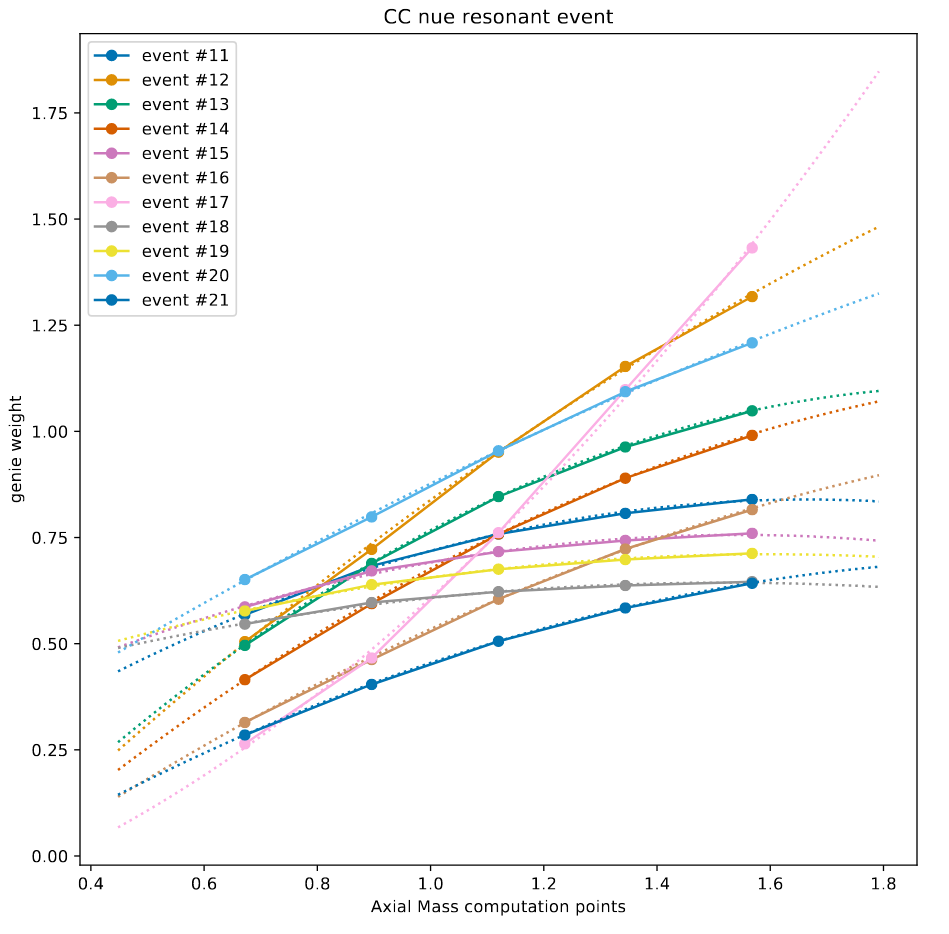
\includegraphics[width=0.5\textwidth]{figures/measurement/systematics/xsec/nue_cc_res_xsec_Ma_systematic.png}
    \caption{Genie interaction weights as a function of the axial mass term systematic $M_{A}$, for 10 $\nu_{e}$ CC events produced via resonance interactions. Each dot represents a discrete point for which the event's cross section is computed in genie. The dashed line represents the quadratic fit made used to interpolate the weight value over the continuous range allowed for the systematic parameter.}
    \label{xsec:resonant_mass}
\end{figure}

\begin{figure}[!t] 
    \centering
    \begin{subfigure}[t]{0.7\textwidth}
        \centering
        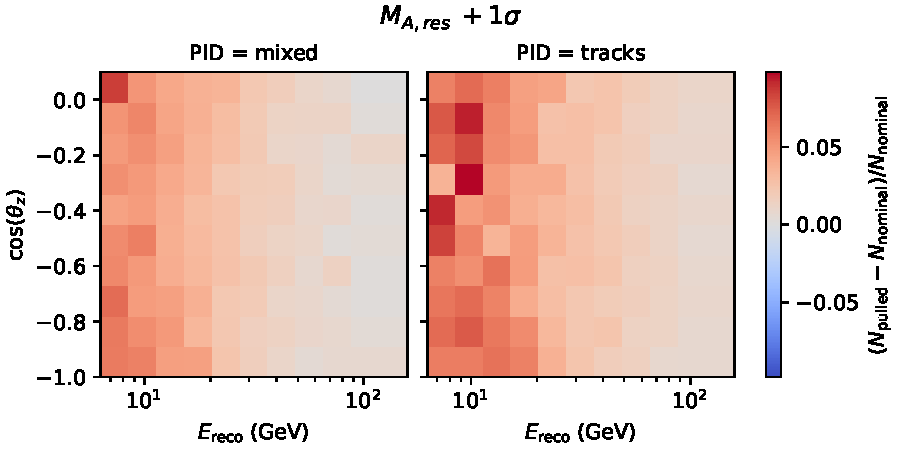
\includegraphics[width=0.99\textwidth,trim={0 0 0 0.6cm},clip]{figures/measurement/systematics/xsec/Genie_Ma_RES.pdf}
        \caption{GENIE $M_{A}^\mathrm{RES}$}
    \end{subfigure}
    \begin{subfigure}[t]{0.7\textwidth}
        \centering
        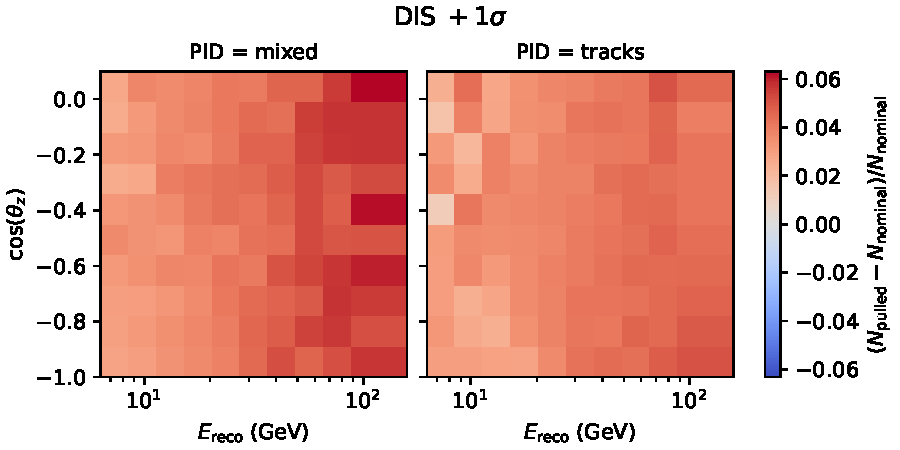
\includegraphics[width=0.99\textwidth,trim={0 0 0 0.6cm},clip]{figures/measurement/systematics/xsec/dis_csms.pdf}
        \caption{DIS CSMS}
    \end{subfigure}  
  \caption{Fractional difference in event rates between (top )$M_{A}^\mathrm{RES}$ (bottom) dis$\_$csms at 1$\sigma$ and at nominal value for both PID bins.
  \label{fig:template_xsecsyst}}
\end{figure}

The uncertainty on the DIS cross-section is primarily given by the disagreement in DIS calculation between CSMS and GENIE cross-sections at energies above 100~GeV. This analysis includes a parameter that interpolates between these two calculations with a linear extrapolation to energies below 100~GeV.
The bottom panel of figure~\ref{fig:template_xsecsyst} illustrates an example of the varying this parameter, DIS, on the final level sample. As expected, the impact of the parameter is largest in the highest energy bins.

There is an additional uncertainty of 20\% on the normalization of NC events to account for uncertainties of the hadronization process and the Weinberg angle.

% Many cross section systematic parameters were tested to see the effect of those on the final verification sample \textcolor{blue}{ and were found to have negligible effect to our analysis so these are not included in this analysis}. A study was performed on the parameters used in the Bodek-Yang model to correct for the parton distribution functions (PDFs) used in the calculation of cross sections in low $Q^2$ region. These DIS events were re-weighted on an event-by-event basis in response to changes in the higher-twist parameters and u valence quark corrections to the GRV98 PDF used in GENIE. Further study was performed on the impact of high-W averaged charged hadronization multiplicity for DIS interactions. It was done by comparing GENIE predictions and bubble chamber data for the averaged charged hadron multiplicity as a function of hadronic mass squared ($W^2$). It was found that modifying PYTHIA6 parameters can achieved better data-MC agreement in the high $W^2$ region.% \cite{Syst_int:PYTHIA6}. 
% Another DIS-related uncertainty studied was its differential cross section. The approach here was to modify the structure function as a function of the Bjorken-x within the uncertainties measured by NuTeV. %\cite{Syst_int:NuTeV}.
% Details of these studies can be found in \href{https://drive.google.com/file/d/1voZ56RCKjDZzPH5qAkvtY3Wkp5EwVi1F/view}{this presentation}.
\subsection{Atmospheric Muons}

Because the muon background contamination is cut to only $\sim$2\%, the impact of muon systematics is generally small. Only the over-all scale is left as a free parameter in the analysis, its impact is shown in figure \ref{fig:weight-scale-syst}. This scale also largely absorbs the effects of DOM efficiency uncertainties, since, to first order, an increase in DOM efficiency leads to a better muon rejection. The spectral index of the muon flux has a very small effect far below the percent-level as shown in figure \ref{fig:delta-gamma-mu-syst} and is therefore kept fixed in the fit.

\begin{figure}[H]
    \centering
    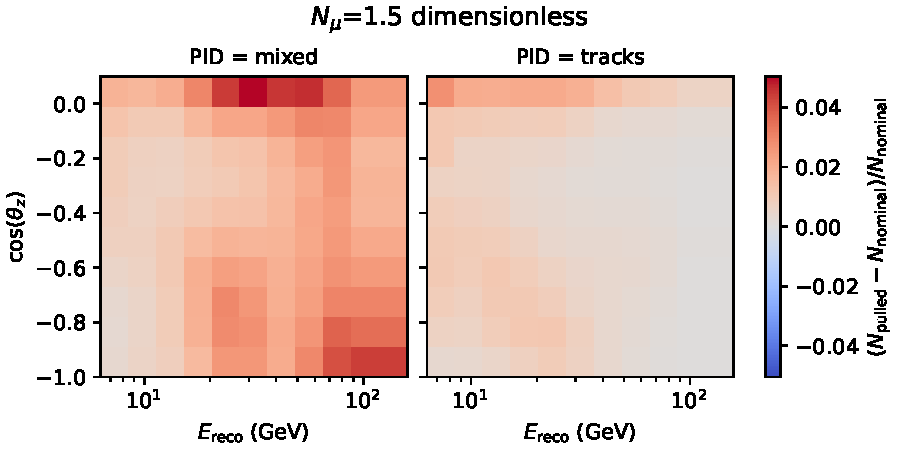
\includegraphics[width=0.7\textwidth,trim={0 0 0 0.6cm},clip]{figures/measurement/systematics/muons/weight_scale.pdf}
    \caption{Impact on the final histograms when the muon normalization is increased by 50\%. The largest impact is seen above the horizon in the mixed PID channel with a change in bin count of 5\%.}
    \label{fig:weight-scale-syst}
\end{figure}

\begin{figure}[H]
    \centering
    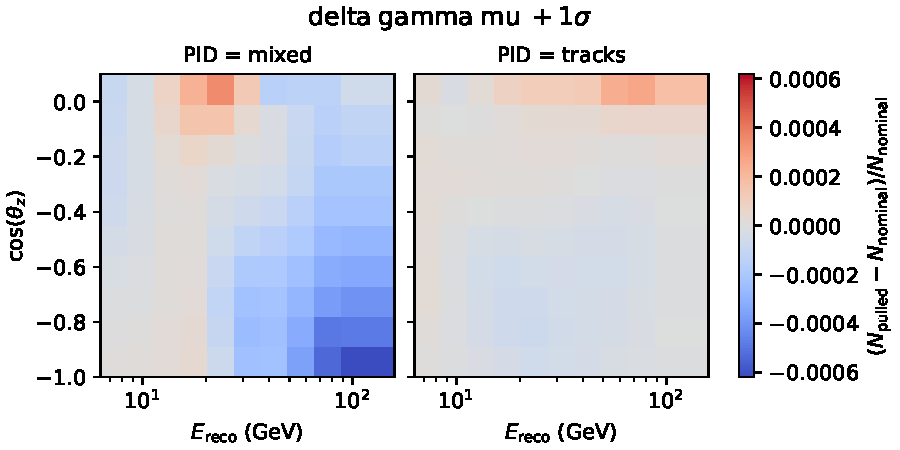
\includegraphics[width=0.7\textwidth,trim={0 0 0 0.6cm},clip]{figures/measurement/systematics/muons/delta_gamma_mu.pdf}
    \caption{Impact on the final histograms when the muon spectral index is increased by $1\sigma$.}
    \label{fig:delta-gamma-mu-syst}
\end{figure}